%% LaTeX-Beamer template for KIT design
%% by Erik Burger, Christian Hammer
%% title picture by Klaus Krogmann
%%
%% version 2.1
%%
%% mostly compatible to KIT corporate design v2.0
%% http://intranet.kit.edu/gestaltungsrichtlinien.php
%%
%% Problems, bugs and comments to
%% burger@kit.edu

\documentclass[18pt]{beamer}

%% SLIDE FORMAT

% use 'beamerthemekit' for standard 4:3 ratio
% for widescreen slides (16:9), use 'beamerthemekitwide'

\usepackage{templates/beamerthemekit}
% \usepackage{templates/beamerthemekitwide}

\usepackage[utf8]{inputenc}
\usepackage{hyperref}
\usepackage{listings}
\usepackage{xcolor}
\usepackage{colortbl}
\usepackage{array}
\usepackage{tikz}
\usetikzlibrary{calc,shapes.multipart,chains,arrows}

\definecolor{lime}{HTML}{8FFF53}

%% TITLE PICTURE

% if a custom picture is to be used on the title page, copy it into the 'logos'
% directory, in the line below, replace 'mypicture' with the
% filename (without extension) and uncomment the following line
% (picture proportions: 63 : 20 for standard, 169 : 40 for wide
% *.eps format if you use latex+dvips+ps2pdf,
% *.jpg/*.png/*.pdf if you use pdflatex)

\titleimage{greendrop}

%% TITLE LOGO

% for a custom logo on the front page, copy your file into the 'logos'
% directory, insert the filename in the line below and uncomment it

%\titlelogo{mylogo}

% (*.eps format if you use latex+dvips+ps2pdf,
% *.jpg/*.png/*.pdf if you use pdflatex)

%% TikZ INTEGRATION

% use these packages for PCM symbols and UML classes
% \usepackage{templates/tikzkit}
% \usepackage{templates/tikzuml}

% the presentation starts here

\title[Sichtbarkeit, Listen, Graphen]{Programmieren:\\ Sichtbarkeit, Listen, Graphen}
\subtitle{Tutorium 30}
\author{YouniS Bensalah}
\date{November 27, 2015}

\institute{Chair for Software Design and Quality}

% Bibliography

\usepackage[citestyle=authoryear,bibstyle=numeric,hyperref,backend=biber]{biblatex}
\addbibresource{templates/example.bib}
\bibhang1em

\begin{document}

% change the following line to "ngerman" for German style date and logos
\selectlanguage{english}

%title page
\begin{frame}
\titlepage
\end{frame}

%table of contents
\begin{frame}{Heute}
\tableofcontents
\end{frame}


\section{Sichtbarkeit und Datenkapselung}

\subsection{Datenkapselung}

\begin{frame}{Datenkapselung}
    \begin{figure}
        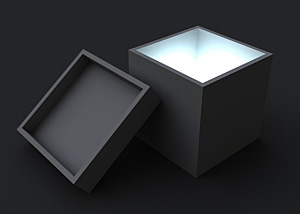
\includegraphics[scale=3.5]{img/most_blackbox.png}
    \end{figure}
\end{frame}


\begin{frame}{Datenkapselung}
    \begin{block}{Datenkapselung}
        \begin{itemize}
            \item Verbergen von Daten oder Informationen vor dem Zugriff von außen
            \item Kein direkter Zugriff auf die interne Datenstruktur
            \item Zugriff nur über feste Schnittstelle
        \end{itemize}
    \end{block}
\end{frame}

\begin{frame}[fragile]{Beispiel: Color}

    Wie es \textit{nicht} geht\dots

    \begin{exampleblock}{}
        \begin{lstlisting}[language=Java]
public class Color {
    public int red;
    public int green;
    public int blue;

    public Color(int red, int green, int blue) { ... }
}

public class Rectangle {
    public void fill(Color c) { ... }
}
        \end{lstlisting}

    \end{exampleblock}

\end{frame}

\begin{frame}[fragile]{Beispiel: Color}

    Hier ist noch alles ok\dots

    \begin{exampleblock}{}
        \begin{lstlisting}[language=Java]
color = new Color(145, 255, 0);
color.blue = 49;

rectangle.fill(color);
        \end{lstlisting}

    \end{exampleblock}

\end{frame}

\begin{frame}[fragile]{Beispiel: Color}

    Hier nicht mehr\dots

    \begin{exampleblock}{}
        \begin{lstlisting}[language=Java]
color = new Color(145, 255, 0);
color.green = -2000;  // whoops

rectangle.fill(color);
        \end{lstlisting}

    \end{exampleblock}

\end{frame}


\begin{frame}[fragile]{Beispiel: Color}

    Was ist, wenn ich lieber eine andere Darstellung möchte\dots

    \begin{exampleblock}{}
        \begin{lstlisting}[language=Java]
public class Color {
    public int hue;
    public int saturation;
    public int value;
}
        \end{lstlisting}

    \end{exampleblock}

\end{frame}

\begin{frame}[fragile]{Beispiel: Color}

    Was ist, wenn ich verschiedene Darstellungen haben möchte\dots

    \begin{exampleblock}{}
        \begin{lstlisting}[language=Java]
public class Color {
    public int hue;
    public int saturation;
    public int value;

    public int red;
    public int green;
    public int blue;
}
        \end{lstlisting}

    \end{exampleblock}

\end{frame}


\begin{frame}{Beispiel: Color}

    \alert{Attribute sind hier \texttt{public} !}

    \begin{itemize}
        \item Keine Kontrolle über die Gültigkeit der Werte in den Attributen
        \item Nutzer der Klasse kann jeden Müll in Attribute schreiben
        \item Innere Darstellung kann nicht transparent geändert werden
        \item Code ist an innere Implementierung gebunden
    \end{itemize}
\end{frame}

\begin{frame}{Beispiel: Color}
    \LARGE{Eine Klasse ist \textbf{keine} Zusammenfassung von verschiedenen Variablen.}

\end{frame}

\begin{frame}[fragile]{Beispiel: Color}
    Wie es eigentlich geht\dots

    \begin{itemize}
        \item Attribute sollten \textbf{private} sein
        \item Kontrollierter Zugriff auf Attribute via \textbf{Getter/Setter}
        \item Keine ungültigen Werte zulassen (in Setter und Konstruktor)
        \item Nutzer der Klasse kennt nur \textbf{genau festgelegte Schnittstelle}
    \end{itemize}
\end{frame}

\begin{frame}{Datenkapselung}
    \textsc{\LARGE{Ignorance is bliss:}}\\
    \textsc{if you do not know about something, you do not worry about it.}
\end{frame}


\subsection{Pakete}

\begin{frame}{Pakete}
    \begin{block}{Paket}
        Ein \textbf{Paket} (\texttt{package}) ist eine Gruppierung von zusammengehörigen Klassen.
    \end{block}
\end{frame}

\begin{frame}{Paket-Deklaration}

    \begin{itemize}
        \item Eine Klasse kann einem Paket zugeordnet werden
        \item Deklaration des Pakets steht am Anfang der Datei
        \item Syntax:\\ \texttt{package} \textit{name}\texttt{;}
        \item Punkt "\texttt{.}" trennt Unterpakete:\\ \texttt{package edu.kit.geometry;}
    \end{itemize}
\end{frame}

\begin{frame}[fragile]{Paket-Deklaration}
    \begin{exampleblock}{Cat.java}
        \begin{lstlisting}[language=Java]
package animals;

public class Cat {
    // ...
}
        \end{lstlisting}

    \end{exampleblock}

\end{frame}



\begin{frame}{Zugriff auf Pakete}
    Wie kann man auf Klasse eines anderen Pakets zugreifen ?
\end{frame}

\begin{frame}[fragile]{Zugriff auf Pakete}
    \begin{exampleblock}{Qualifizierter Name}
        \begin{lstlisting}[language=Java]
animals.Cat garfield = new animals.Cat();
        \end{lstlisting}

    \end{exampleblock}

\end{frame}

\begin{frame}[fragile]{Zugriff auf Pakete}
    \begin{exampleblock}{Klasse importieren}
        \begin{lstlisting}[language=Java]
import animals.Cat;

Cat garfield = new Cat();
        \end{lstlisting}

    \end{exampleblock}

\end{frame}

\begin{frame}[fragile]{Zugriff auf Pakete}
    \begin{exampleblock}{Paket importieren}
        \begin{lstlisting}[language=Java]
import animals.*;

Cat garfield = new Cat();
Dog odie = new Dog();
Fish nemo = new Fish();
        \end{lstlisting}

    \end{exampleblock}

\end{frame}

\begin{frame}[fragile]{Paket- und Ordnerstruktur}

    \begin{columns}[c]

        \column{.5\textwidth}
        \begin{exampleblock}{Paketstruktur}
            \begin{lstlisting}[basicstyle=\scriptsize]
math

    math.geometry
        math.geometry.Vector
        math.geometry.Sphere
        math.geometry.Cube

    math.algebra
        math.algebra.Group
        math.algebra.Ring
        math.algebra.Field

    math.BigNumber
            \end{lstlisting}

        \end{exampleblock}

        \column{.5\textwidth}
        \begin{exampleblock}{Ordnerstruktur}
            \begin{lstlisting}[basicstyle=\scriptsize]
math/

    geometry/
        Vector.java
        Sphere.java
        Cube.java

    algebra/
        Group.java
        Ring.java
        Field.java

    BigNumber.java
            \end{lstlisting}
        \end{exampleblock}

    \end{columns}

    \vspace{.2in}

    \textbf{Konvention:} Paket- und Ordnerstruktur sollten übereinstimmen

\end{frame}



\subsection{Sichtbarkeitsmodifizierer}

\begin{frame}{Sichtbarkeitsmodifizierer}

    \begin{itemize}
        \item \texttt{public}\\ Sichtbar für alle
        \item \texttt{-}\\ Nur innerhalb des Pakets sichtbar
        \item \texttt{private}\\ Nur innerhalb der Klasse sichtbar
    \end{itemize}
\end{frame}


\section{Listen und abstrakte Datentypen}

\begin{frame}{Listen und abstrakte Datentypen}
    \begin{figure}
        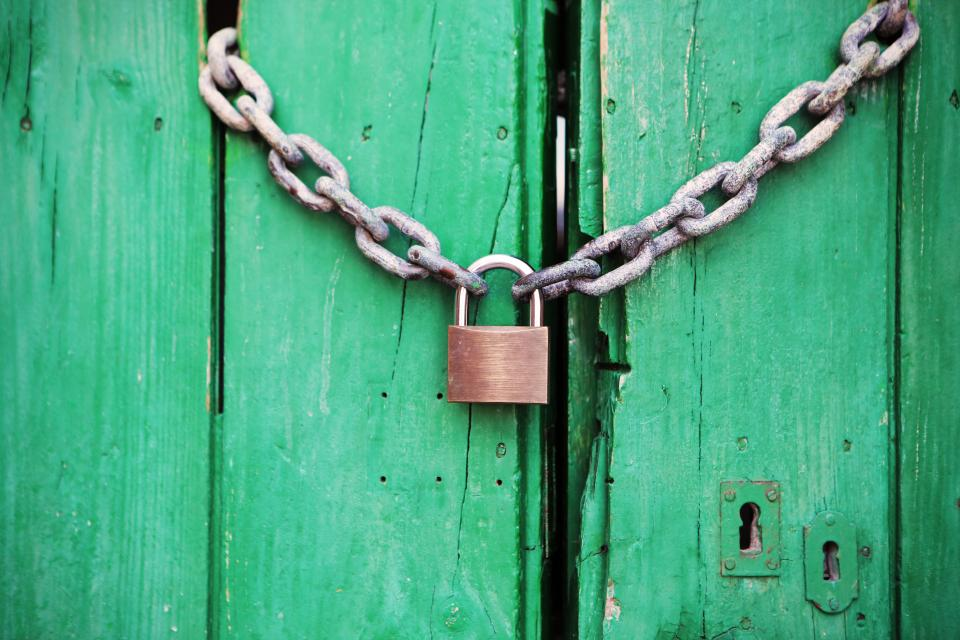
\includegraphics[scale=.3]{img/AD76394B17.jpg}
    \end{figure}
\end{frame}

\begin{frame}{Rekursive Datentypen}
    \begin{block}{Rekursiver Datentyp}
        Ein Datentyp ist \textit{rekursiv}, wenn Objekte Verweise auf Objekte derselben Klasse enthalten.
    \end{block}
\end{frame}


\subsection{Verkettete Listen}

\begin{frame}{Verkettete Listen}
    \begin{block}{Verkettete Listen}
        Eine \textbf{verkettete Liste} ist eine dynamische Datenstruktur, bei der jedes Element auf seinen Nachbarn verweist.
    \end{block}

\end{frame}

\begin{frame}{Verkettete Listen}
    Verkettete Listen sind ein \textit{rekursiver Datentyp}.
\end{frame}

\begin{frame}{Einfach Verkettete Listen}

    \begin{itemize}
        \item Bei einer \textbf{einfach verketteten Liste} zeigt jedes Element auf das nächste Element in der Liste.
        \item Jedes Element enthält auch den eigentlichen Inhalt der Zelle.
        \item Das letzte Element zeigt auf \texttt{null}.
    \end{itemize}

    \begin{figure}
        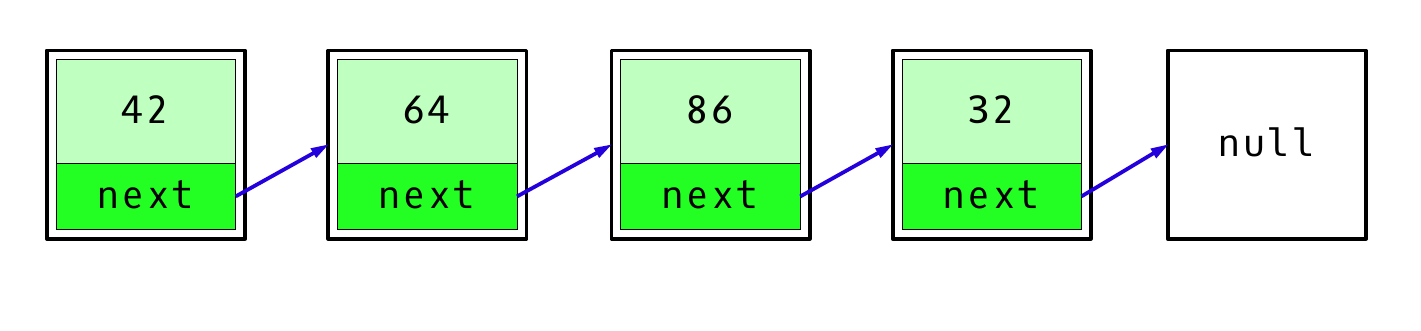
\includegraphics[scale=.3]{img/simplelinkedlist.png}
    \end{figure}

\end{frame}

\begin{frame}[fragile]{Einfach Verkettete Listen}

    Implementierung in Java\dots

    \begin{exampleblock}{}
        \begin{lstlisting}[language=Java,basicstyle=\scriptsize]
public class Cell {
    private int content;
    private Cell next;
}
        \end{lstlisting}
    \end{exampleblock}

\end{frame}

\begin{frame}[fragile]{Einfach Verkettete Listen}

    \begin{exampleblock}{}
        \begin{lstlisting}[language=Java,basicstyle=\scriptsize]
public class Cell {
    private int content;
    private Cell next;

    public Cell(int content, Cell next) {
        this.content = content;
        this.next = next;
    }

    public Cell getNext() { return this.next; }
    public void setNext(Cell next) { this.next = next; }
    public int getContent() { return this.content; }
    public void setContent(int content) { this.content = content; }
}
        \end{lstlisting}
    \end{exampleblock}

\end{frame}


\begin{frame}[fragile]{Einfach Verkettete Listen}

    \begin{exampleblock}{}
        \begin{lstlisting}[language=Java,basicstyle=\scriptsize]
Cell c3 = new Cell(32, null);    // c3 --> null
Cell c2 = new Cell(99, c3);      // c2 --> c3
Cell c1 = new Cell(42, c2);      // c1 --> c2
        \end{lstlisting}
    \end{exampleblock}

\vspace{.2in}

\pause

Das erste Element (\texttt{head}) genügt, um komplette Liste zu durchlaufen !

\end{frame}


\begin{frame}{Operationen auf verketteten Listen}
    \begin{itemize}
        \item \textbf{Einfügen} von Listenelementen\\
        \texttt{addFirst}, \texttt{addLast}
        \item \textbf{Löschen} von Listenelementen\\
        \texttt{remove}
        \item \textbf{Suchen} nach Listenelementen\\
        \texttt{contains}
        \item \dots
    \end{itemize}
\end{frame}

\begin{frame}[fragile]{Operationen auf verketteten Listen}
    Wir fassen nun die aneinanderhängenden Listenelemente zu einer Klasse \textbf{Liste} zusammen.

    \begin{exampleblock}{}
        \begin{lstlisting}[language=Java,basicstyle=\scriptsize]
public class List {
    private Cell head;

    public List(Cell head) {
        this.head = head;
    }
}
        \end{lstlisting}

    \end{exampleblock}


\end{frame}

\begin{frame}{Einfügen}
    \textbf{Einfügen} von Listenelementen an Anfang oder Ende der Liste
\end{frame}


\begin{frame}[fragile]{Einfügen}
    \begin{exampleblock}{addFirst}
        \begin{lstlisting}[language=Java,basicstyle=\scriptsize]
public void addFirst(int content) {
    Cell c = new Cell(content, this.head);
    this.head = c;
}
        \end{lstlisting}

    \end{exampleblock}

\end{frame}

\begin{frame}[fragile]{Einfügen}

    \begin{exampleblock}{addLast}
        \begin{lstlisting}[language=Java,basicstyle=\scriptsize]
public void addLast(int content) {
    if (this.head == null) {
        this.head = new Cell(content, null);
        return;
    }

    Cell c = this.head;
    while (c.getNext() != null) {
        c = c.getNext();
    }
    c.setNext(new Cell(content, null));
}
        \end{lstlisting}

    \end{exampleblock}

\end{frame}

\begin{frame}{Löschen}
    \textbf{Löschen} von Listenelementen
\end{frame}

\begin{frame}[fragile]{Löschen}
    \begin{exampleblock}{remove}
        \begin{lstlisting}[language=Java,basicstyle=\scriptsize]
public void remove(int content) {
    Cell c = this.head;

    while (c != null && c.getContent() == content) {
        this.head = c.getNext();
        c = this.head;
    }

    if (c == null) {
        return;
    }

    while (c.getNext() != null) {
        if (c.getNext().getContent() == content) {
            c.setNext(c.getNext().getNext());
        } else {
            c = c.getNext();
        }
    }
}
        \end{lstlisting}

    \end{exampleblock}

\end{frame}

\begin{frame}{Suchen}
    \textbf{Suchen} nach Listenelementen
\end{frame}

\begin{frame}[fragile]{Suchen}
    \begin{exampleblock}{contains}
        \begin{lstlisting}[language=Java,basicstyle=\scriptsize]
public boolean contains(int content) {
    for (Cell c = this.head; c != null; c = c.getNext()) {
        if (c.getContent() == content) {
            return true;
        }
    }
    return false;
}
        \end{lstlisting}

    \end{exampleblock}

\end{frame}


\begin{frame}{Doppelt Verkettete Listen}
    \begin{itemize}
        \item Jedes \textbf{Listenelement} merkt sich sowohl das \textbf{nächste} (\texttt{next}) als auch das \textbf{vorherige} (\texttt{prev}) Element
        \item \textbf{Liste} merkt sich dann sowohl \textbf{Anfang} (\texttt{head}) als auch \textbf{Ende} (\texttt{tail}) der Liste
        \item Liste kann \textit{vorwärts} wie \textit{rückwärts} traversiert werden
        \item \texttt{addLast}-Operation jetzt in $\mathcal{O}(1)$ möglich !
    \end{itemize}

    \begin{figure}
        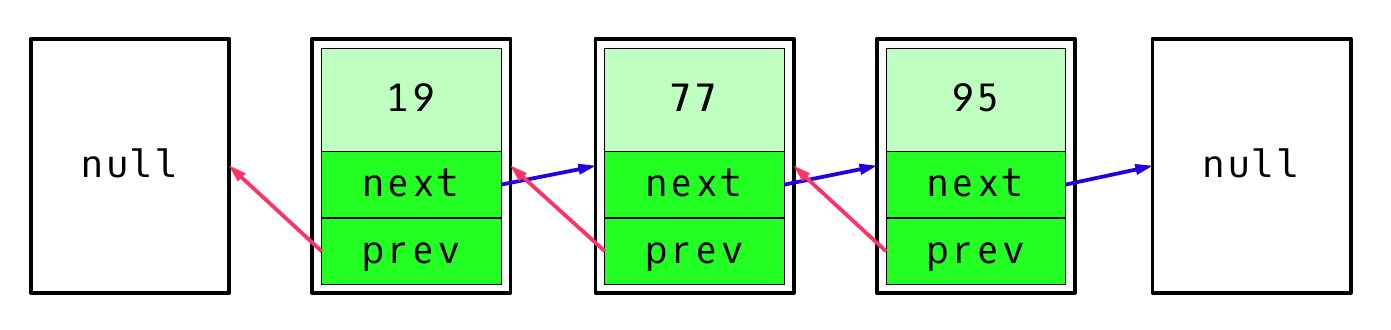
\includegraphics[scale=.3]{img/doublelinkedlist.png}
    \end{figure}
\end{frame}

\begin{frame}{Listen vs. Arrays}
    \begin{itemize}
        \item \textbf{Listen}
        \begin{itemize}
            \item Dynamische Größe
            \item Einfaches Einfügen und Löschen von Elementen
            \item Zugriff auf innere Elemente nur durch Traversierung der Liste möglich
        \end{itemize}
        \item \textbf{Arrays}
        \begin{itemize}
            \item Statische Größe
            \item Einfacher Zugriff auf beliebige Elemente in $\mathcal{O}(1)$
            \item Cache-effizient
        \end{itemize}
    \end{itemize}
\end{frame}


\subsection{Abstrakte Datentypen}

\begin{frame}{Abstrakte Datentypen}
    \begin{block}{Abstrakter Datentyp}
        Ein \textbf{abstrakter Datentyp} beschreibt eine Menge von Typen in Kombination mit zulässigen Operationen.
    \end{block}

\end{frame}

\begin{frame}{Abstrakte Datentypen}
    \begin{itemize}
        \item \textbf{Geheimnisprinzip}:\\
        Wenn wir eine Liste nur als solche verwenden wollen,
        interessiert uns der interne Aufbau der Liste eigentlich gar nicht
        \item Abstrakte Sicht auf die Liste
    \end{itemize}

\end{frame}


\begin{frame}{Abstrakte Datentypen}
    \begin{alertblock}{Datenkapselung}
        \begin{itemize}
            \item Ein abstrakter Datentyp trifft \textit{keine} Aussagen über konkrete Implementierung
            \item Prinzip der Datenkapselung
            \item Zugriff auf Inhalt der Liste nur über definierte Schnittstelle
        \end{itemize}
    \end{alertblock}

\end{frame}

\subsection{Iteratoren}


\begin{frame}{Iteratoren}
    \begin{block}{Iterator}
        Ein \textbf{Iterator} ist ein Zeiger, mit dem die Elemente einer Datenstruktur (z. B. Liste) durchlaufen werden können.
    \end{block}

\end{frame}

\begin{frame}[fragile]{Iteratoren}

    \begin{exampleblock}{Iterator für Liste}
        \begin{lstlisting}[language=Java,basicstyle=\scriptsize]
public class List {
    // ...
    public class Iterator {
        private Cell cursor;
        private Iterator(Cell start) { this.cursor = start; }
        public boolean hasNext() { return this.cursor != null; }
        public int next() {
            int c = this.cursor.getContent();
            this.cursor = this.cursor.getNext();
            return c;
        }
    }

    public Iterator iterator() {
        return new Iterator(this.head);
    }
}
        \end{lstlisting}

    \end{exampleblock}


\end{frame}

\begin{frame}[fragile]{Iteratoren}

    \begin{exampleblock}{Verwendung eines Iterators}
        \begin{lstlisting}[language=Java,basicstyle=\scriptsize]
List myList;
// ...

List.Iterator it = myList.iterator();
while (it.hasNext()) {
    int x = it.next();
    doWork(x);
}
        \end{lstlisting}

    \end{exampleblock}


\end{frame}

\section{Graphen}

\subsection{Knoten und Kanten}

\begin{frame}{Graphen}
    \begin{figure}
        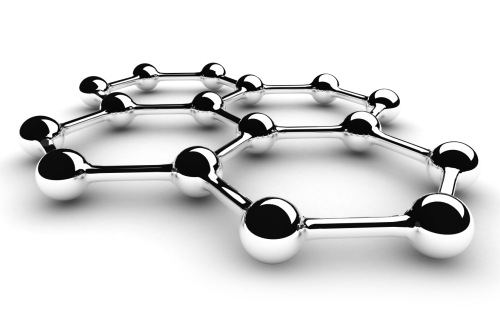
\includegraphics[scale=2.5]{img/graph.jpg}
    \end{figure}
\end{frame}

\begin{frame}{Graphen}
    \begin{block}{Definition}
        Ein \textbf{Graph} ist ein Paar $\mathcal{G} = (\mathcal{V}, \mathcal{E})$
        mit $\mathcal{V}$ Menge von Knoten
        und $\mathcal{E} \subset \mathcal{V} \times \mathcal{V}$ Menge von Kanten.
    \end{block}

\end{frame}


\begin{frame}{Graphen}
        \begin{figure}
            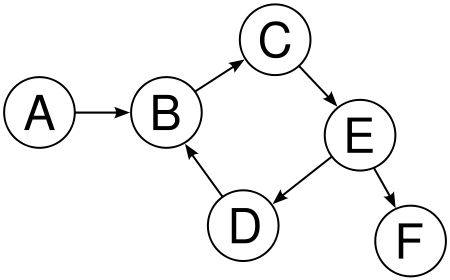
\includegraphics[scale=.5]{img/graph.png}
        \end{figure}

\end{frame}


\begin{frame}{Graphen}

        \begin{exampleblock}{}
            \begin{itemize}
                \item $\mathcal{V} = $ ?
                \item $\mathcal{E} = $ ?
            \end{itemize}
        \end{exampleblock}


        \begin{figure}
            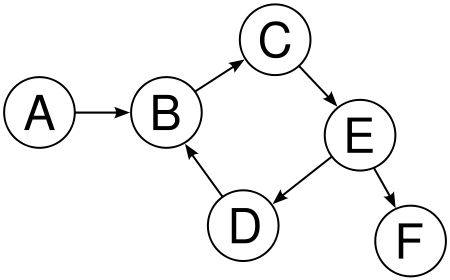
\includegraphics[scale=.3]{img/graph.png}
        \end{figure}

\end{frame}

\begin{frame}{Graphen}

        \begin{exampleblock}{}
            \begin{itemize}
                \item $\mathcal{V} = \left\{ A, B, C, D, E, F \right\}$
                \item $\mathcal{E} = \left\{ (A, B), (B, C), (C, E), (D, B), (E, D), (E, F) \right\}$
            \end{itemize}
        \end{exampleblock}


        \begin{figure}
            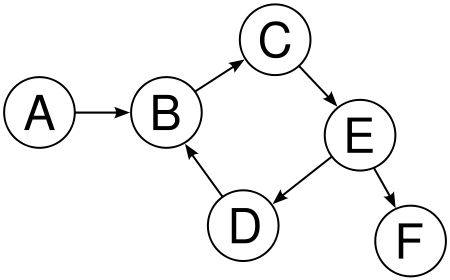
\includegraphics[scale=.3]{img/graph.png}
        \end{figure}

\end{frame}

\begin{frame}{Darstellung von Graphen}
    \textbf{Problem:} Wie kann ich einen Graphen in meinem Programm darstellen ?
\end{frame}


\subsection{Adjazenzmatrix}

\begin{frame}{Adjazenzmatrix}
    \[
    \left(
    \begin{array}{cccccc}
        0 & 1 & 0 & 0 & 0 & 0 \\
        0 & 0 & 1 & 0 & 0 & 0 \\
        0 & 0 & 0 & 0 & 1 & 0 \\
        0 & 1 & 0 & 0 & 0 & 0 \\
        0 & 0 & 0 & 1 & 0 & 1 \\
        0 & 0 & 0 & 0 & 0 & 0
    \end{array}
    \right)
    \]

    \begin{figure}
        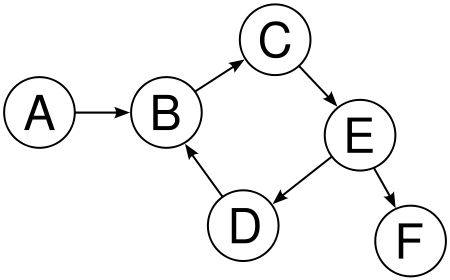
\includegraphics[scale=.3]{img/graph.png}
    \end{figure}

\end{frame}


\begin{frame}{Adjazenzmatrix}
    \[
    \left(
    \begin{array}{cccccc}
        0 & 1 & 0 & 0 & 0 & 0 \\
        0 & 0 & 1 & 0 & 0 & 0 \\
        0 & 0 & 0 & 0 & 1 & 0 \\
        0 & 1 & 0 & 0 & 0 & 0 \\
        0 & 0 & 0 & 1 & 0 & 1 \\
        0 & 0 & 0 & 0 & 0 & 0
    \end{array}
    \right)
    \]

    \begin{itemize}
        \item Adjazenzmatrix speichert, welche Knoten des Graphen durch eine Kante verbunden sind
        \item Zeilen entsprechen den Startknoten, Spalten entsprechen den Zielknoten
        \item $1$ bedeutet, dass eine Kante existiert, $0$ bedeutet, dass die Knoten \textit{nicht} verbunden sind
    \end{itemize}

\end{frame}

\appendix
\beginbackup

\begin{frame}[fragile]{String.split}
    \begin{lstlisting}[language=Java]
String[] split(String regex)
    \end{lstlisting}


    \begin{itemize}
        \item \texttt{String.split} zerlegt eine Zeichenkette nach einem gegebenen Muster
        \item Als Rückgabe erhält man einen Array mit den einzelnen Stücken
    \end{itemize}

\begin{exampleblock}{}
    \begin{lstlisting}[language=Java,basicstyle=\scriptsize]
String[] result = String.split(";", "cyan;yellow;magenta");
    \end{lstlisting}
\end{exampleblock}

\begin{itemize}
    \item Der Array \texttt{result} enthält jetzt\\ \texttt{\{ "cyan", "yellow", "magenta" \}}
\end{itemize}

\end{frame}

\begin{frame}{Gleichheit von Objekten}
    \begin{itemize}
        \item In Java gibt es zwei Möglichkeiten, auf Gleichheit zu prüfen
        \begin{itemize}
            \item \texttt{"=="}\\
            Prüft auf Wert-Gleichheit

            \item \texttt{equals}\\
            Prüft auf inhaltliche Objekt-Gleichheit
        \end{itemize}
        \item Klasse kann \texttt{equals}-Methode \textbf{überladen} und Gleichheit von zwei Objekten selbst definieren
        \item \alert{Bei \textbf{Objekten} ist Wert-Gleichheit gerade \textbf{Gleichheit der Referenz} !}
    \end{itemize}
\end{frame}


\begin{frame}{Fragen ?}
    \begin{figure}
        
\includegraphics[scale=.7]{img/formulas.png}
    \end{figure}
\end{frame}

\begin{frame}{Bis nächste Woche !}
    \begin{figure}
        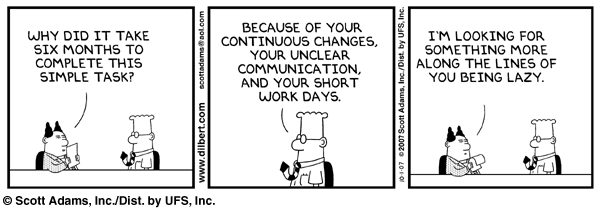
\includegraphics[scale=.5]{img/dilbert2733310071001kc4.png}
    \end{figure}

    \begin{flushright}
    \footnotesize{xkcd.com}
    \end{flushright}
\end{frame}

\backupend

\end{document}
